\cleardoublepage
\chapter{PENGEMBANGAN SISTEM KOREKSI TARIF PAJAK PENGHASILAN BERBASIS AI PADA WEB TUKAR FAKTUR}
\label{chap:judul-pekerjaan}

\section{Deskripsi Persoalan}
\label{sec:deskripsi_persoalan}

Proses pengadaan barang dan jasa di PT Paragon Technology and Innovation melibatkan pencatatan transaksi pada SAP serta pemeriksaan dokumen tagihan melalui \textit{Web Tukar Faktur}.
Salah satu aspek yang diperiksa adalah kesesuaian kode internal SAP yang menentukan kategori Pajak Penghasilan (PPh) pada transaksi, yaitu \textit{WHT code}.
Kode tersebut menjadi dasar penentuan tarif untuk menghitung PPh yang perlu dibayarkan oleh Paragon dalam transaksi terkait.
Dengan demikian, ketepatan \textit{WHT code} bergantung pada kesesuaian data transaksi yang digunakan dalam proses penentuannya.

Alur pengadaan dimulai ketika pengguna membuat \textit{purchase request} (PR) untuk mengajukan kebutuhan barang atau jasa.
Pada tahap ini, pengguna memilih \textit{material group}, yaitu kelompok yang merepresentasikan kategori barang atau jasa yang diajukan.
PR kemudian diperiksa oleh pihak yang bertanggung jawab memberikan persetujuan sebelum diproses menjadi \textit{purchase order} (PO).
Dalam kondisi yang menjadi persoalan, pengguna kerap memilih \textit{material group} yang tidak sesuai dengan barang atau jasa yang sebenarnya dibeli.
Ketidaksesuaian tersebut tidak selalu teridentifikasi pada tahap pemeriksaan PR sehingga pengajuan tetap disetujui dan kesalahan terbawa hingga ke PO.

SAP menentukan \textit{WHT code} melalui pemetaan berbasis aturan (\textit{rule-based}) yang bersifat tetap dalam sistem internal perusahaan.
Pemetaan ini menggunakan kombinasi atribut transaksi dan pemasok sebagai masukan.
Atribut-atribut yang digunakan adalah sebagai berikut.
\begin{enumerate}
    \item \textit{Material group}, yaitu kelompok barang atau jasa yang dipilih dalam proses pengadaan dan diteruskan ke PO.
    \item \textit{Legal form}, yaitu bentuk pemasok yang membedakan antara badan dan perorangan.
    \item \textit{Identification number}, yaitu atribut yang memuat informasi surat atau keterangan perpajakan yang berlaku bagi pemasok, misalnya surat keterangan pajak usaha mikro, kecil, dan menengah (UMKM). Atribut ini dapat kosong apabila tidak terdapat surat atau keterangan yang terkait.
    \item \textit{Construction service classification}, yaitu jenis perusahaan konstruksi. Atribut ini dapat kosong.
    \item \textit{Entity country}, yaitu negara tempat entitas atau anak perusahaan Paragon yang melakukan transaksi berada, seperti Indonesia atau Malaysia.
    \item \textit{Vendor country}, yaitu negara asal pemasok yang bertransaksi dengan entitas Paragon.
\end{enumerate}

Dalam mekanisme tersebut, \textit{material group} merupakan salah satu masukan yang memengaruhi hasil pemetaan \textit{WHT code}.
Apabila kelompok yang dipilih tidak sesuai dengan karakteristik barang atau jasa pada transaksi, SAP dapat menghasilkan kode yang sesuai dengan aturan pemetaan, tetapi tidak sesuai dengan substansi transaksi yang sebenarnya.
Oleh karena itu, persoalan yang dihadapi terletak pada ketepatan masukan yang digunakan oleh aturan tersebut.
Kesalahan pada \textit{material group} berpotensi menghasilkan kategori PPh yang tidak tepat dan selanjutnya memengaruhi tarif serta jumlah pajak yang dihitung.

Ketidaksesuaian tersebut diperiksa kembali pada tahap tukar faktur.
Pemasok mengirimkan faktur atau \textit{invoice}, dokumen penerimaan barang atau \textit{goods receipt} (GR), serta dokumen pendukung lainnya kepada bagian \textit{account payable} (AP).
Melalui \textit{Web Tukar Faktur}, AP memeriksa kesesuaian \textit{WHT code} dengan membandingkan barang atau jasa pada setiap item faktur terhadap \textit{material group} yang tercatat di SAP.
Pemeriksaan ini diperlukan karena kode yang telah ditentukan oleh SAP belum tentu mencerminkan transaksi sebenarnya apabila data pengadaan sejak awal tidak tepat.

Apabila hasil pemeriksaan menunjukkan bahwa \textit{WHT code} sudah benar, transaksi dapat dilanjutkan ke tahap pembukuan jurnal (\textit{posting}) pada SAP.
Sebaliknya, apabila kode dinilai belum sesuai, transaksi harus melalui peninjauan perpajakan terlebih dahulu.
Dokumen kemudian dikirim ke tabel penampungan sementara (\textit{staging table}) SAP sebagai \textit{parked document}, yaitu dokumen yang disimpan sementara sebelum pembukuan jurnal diselesaikan.
Koreksi \textit{WHT code} dilakukan secara manual pada tabel tersebut, kemudian transaksi diteruskan ke tahap pembukuan jurnal setelah koreksi selesai.
Dengan demikian, ketidaksesuaian yang berasal dari tahap pengajuan pengadaan menimbulkan pekerjaan tambahan pada tahap pemrosesan faktur.

Alur kondisi saat ini, mulai dari pembuatan PR hingga pembukuan jurnal setelah pemeriksaan \textit{WHT code}, ditunjukkan pada Gambar \ref{fig:sistem-as-is}.

\begin{figure}[htbp]
    \centering
    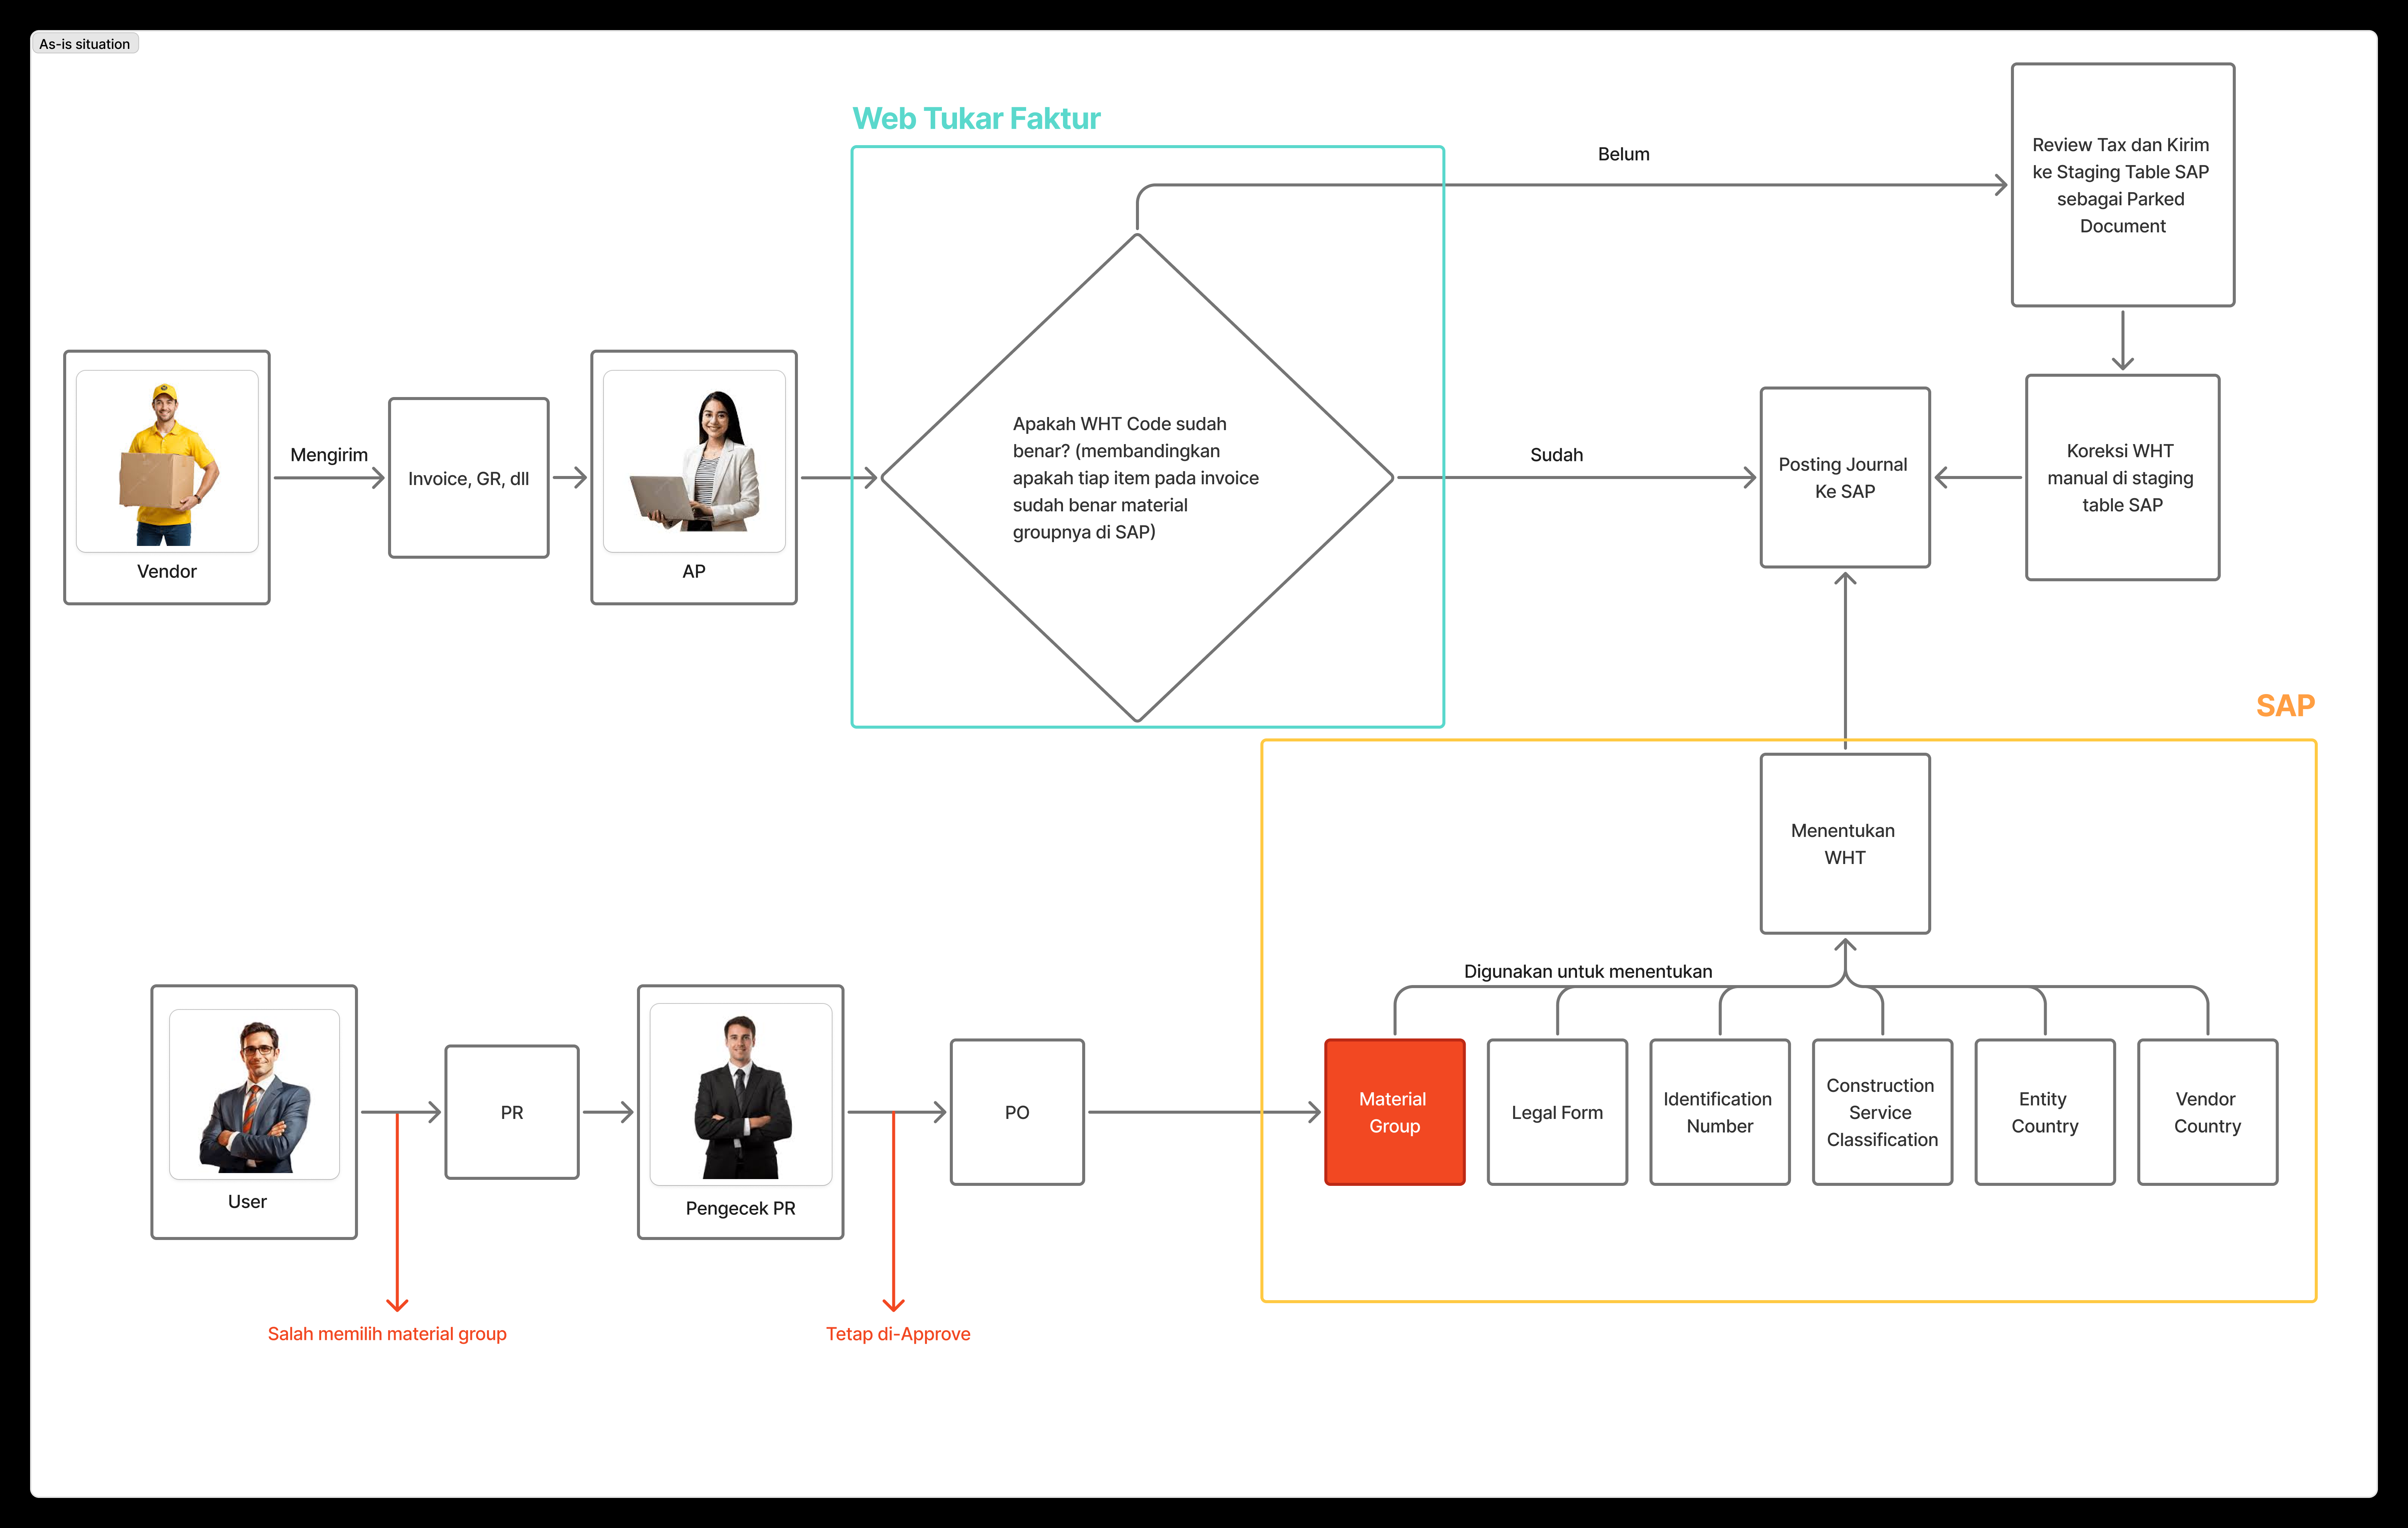
\includegraphics[width=\textwidth]{images/sistem as-is.png}
    \caption{Alur kondisi saat ini dalam penentuan dan koreksi \textit{WHT code}}
    \label{fig:sistem-as-is}
\end{figure}

Alur pemeriksaan dan koreksi tersebut menuntut AP untuk memahami isi setiap item faktur serta menilai kesesuaiannya dengan data yang tercatat di SAP.
Ketika ditemukan kesalahan, diperlukan pula tindak lanjut peninjauan perpajakan dan perubahan kode secara manual sebelum transaksi dapat dibukukan.
Kondisi ini menambah beban pemeriksaan dan dapat memperpanjang waktu pemrosesan faktur.
Apabila ketidaksesuaian tidak teridentifikasi, perhitungan PPh berpotensi tetap menggunakan kategori dan tarif yang tidak sesuai dengan transaksi.

Berdasarkan kondisi tersebut, persoalan utama dalam pekerjaan ini adalah bagaimana membantu proses identifikasi dan koreksi \textit{WHT code} pada tahap tukar faktur ketika \textit{material group} dari proses pengadaan tidak mencerminkan barang atau jasa yang sebenarnya.
Penanganan persoalan perlu mempertimbangkan isi faktur beserta atribut lain yang digunakan dalam pemetaan SAP agar penilaian tidak hanya bergantung pada \textit{material group} yang telah tercatat.
Sesuai dengan ruang lingkup kerja praktik, kebutuhan tersebut menjadi dasar pengembangan sistem berbasis akal imitasi (AI) pada \textit{Web Tukar Faktur} untuk mendukung pemeriksaan dan rekomendasi koreksi \textit{WHT code} sebagai dasar penentuan tarif PPh.

\section{Proses Pengerjaan Sistem Koreksi \textit{WHT Code}}
\label{sec:proses_pengerjaan}

\subsection{Analisis Kebutuhan dan Ruang Lingkup}
\label{subsec:analisis_kebutuhan_ruang_lingkup}

Tahap awal pekerjaan dilakukan melalui pemahaman terhadap proses bisnis tukar faktur, pihak-pihak yang terlibat, serta titik munculnya ketidaksesuaian \textit{WHT code}.
Analisis berfokus pada hubungan antara data yang tercatat pada proses pengadaan, isi dokumen faktur, dan pemeriksaan yang dilakukan oleh AP sebelum transaksi dibukukan pada SAP.
Hasil analisis menunjukkan bahwa kesalahan pemilihan \textit{material group} pada tahap PR dapat tetap terbawa hingga menjadi PO, sedangkan ketidaksesuaian baru teridentifikasi ketika AP membandingkan item faktur dengan data pada SAP.
Oleh sebab itu, sistem yang dikembangkan diarahkan untuk membantu pemeriksaan pada tahap tukar faktur, yaitu saat informasi mengenai transaksi dan dokumen tagihan tersedia.

Secara ideal, penyelesaian persoalan dilakukan pada akar masalah, yaitu dengan mencegah pengguna memilih \textit{material group} yang keliru saat membuat PR.
Namun, perubahan pada tahap tersebut berada di luar ruang lingkup \textit{Web Tukar Faktur} dan memerlukan \textit{change management} yang tinggi karena melibatkan penyesuaian proses kerja serta pemangku kepentingan lintas unit.
Atas pertimbangan tersebut, pengembangan difokuskan pada pengendalian di tahap tukar faktur sebagai titik yang masih berada dalam cakupan unit kerja penulis.

Kebutuhan utama sistem adalah mengidentifikasi potensi ketidaksesuaian \textit{WHT code} secara lebih efisien.
Sistem juga dirancang untuk menggantikan sebagian pemeriksaan manual oleh AP.
Sistem perlu mampu menggunakan konteks barang atau jasa dalam faktur bersama atribut yang digunakan oleh pemetaan SAP, yaitu \textit{material group}, \textit{legal form}, \textit{identification number}, \textit{construction service classification}, \textit{entity country}, dan \textit{vendor country}.
Berdasarkan informasi tersebut, sistem diharapkan dapat menghasilkan rekomendasi \textit{WHT code} beserta tingkat keyakinan (\textit{confidence}) atas rekomendasi tersebut.
Rekomendasi ini ditujukan untuk menilai kesesuaian data transaksi, terutama ketika \textit{material group} yang tercatat tidak selaras dengan barang atau jasa pada faktur.

Tingkat keyakinan digunakan untuk menentukan mekanisme tindak lanjut terhadap suatu faktur.
Apabila sistem menghasilkan rekomendasi dengan tingkat keyakinan tinggi sesuai ambang batas yang ditetapkan, faktur dapat diteruskan ke proses \textit{autopost} tanpa memerlukan campur tangan AP.
Sebaliknya, faktur dengan tingkat keyakinan yang belum memadai tetap diteruskan kepada AP untuk diperiksa dan, apabila diperlukan, ditinjau lebih lanjut oleh pihak perpajakan.
Dengan mekanisme tersebut, sistem secara parsial menggantikan pemeriksaan manual AP pada transaksi yang memiliki tingkat keyakinan tinggi, sambil tetap menyediakan pemeriksaan manusia bagi transaksi yang memerlukan pertimbangan lebih lanjut.

Ruang lingkup pekerjaan dibatasi pada pengembangan subsistem koreksi tarif PPh pada \textit{Web Tukar Faktur}.
Subsistem mencakup pengolahan informasi faktur dan atribut transaksi yang relevan untuk membentuk rekomendasi \textit{WHT code} pada tahap pemeriksaan faktur.
Perubahan terhadap aturan pemetaan \textit{WHT code} yang telah berlaku di SAP, kebijakan perpajakan perusahaan, serta alur pembuatan dan persetujuan PR maupun PO tidak termasuk dalam ruang lingkup pekerjaan.
Pembatasan ini ditetapkan karena proses tersebut berada di luar cakupan unit kerja penulis dan perubahan pada proses tersebut membutuhkan \textit{change management} lintas unit.

Dengan batasan tersebut, keluaran yang diharapkan dari pekerjaan ini adalah suatu kemampuan pada \textit{Web Tukar Faktur} untuk menilai kesesuaian \textit{WHT code} terhadap substansi transaksi sebelum pembukuan jurnal dilakukan.
Kemampuan tersebut diharapkan dapat meneruskan faktur dengan rekomendasi berkeyakinan tinggi ke proses \textit{autopost}, mengarahkan kasus lain kepada AP untuk diperiksa, mengurangi kebutuhan koreksi manual pada tahap akhir proses, dan membantu menjaga ketepatan kategori PPh yang digunakan dalam perhitungan pajak.

\subsection{\textit{Exploratory Data Analysis} dan Perumusan Pendekatan}
\label{subsec:eda_perumusan_pendekatan}

Tahap \textit{exploratory data analysis} (EDA) dilakukan untuk memahami skala, struktur, dan pola pada data yang digunakan dalam penentuan \textit{WHT code}.
Penulis memperoleh dua kelompok data utama.
Data pertama adalah referensi \textit{material group} yang memuat kode, deskripsi, dan contoh penggunaan untuk 636 \textit{material group}.
Data kedua adalah data pemetaan \textit{WHT code} yang terdiri atas 46.660 baris.
Jumlah baris pemetaan tersebut terutama dipengaruhi oleh banyaknya \textit{material group} yang dipetakan terhadap kombinasi atribut transaksi, sehingga tidak seluruh baris merepresentasikan aturan yang berbeda.

Hipotesis awal yang dirumuskan bersama mentor adalah membangun model klasifikasi \textit{material group} berbasis \textit{encoder}, seperti \textit{Bidirectional Encoder Representations from Transformers} (BERT).
Model tersebut diharapkan dapat mengklasifikasikan konteks barang atau jasa pada item faktur ke dalam \textit{material group} yang sesuai.
Namun, pengembangan pendekatan ini membutuhkan sumber daya komputasi, waktu, dan pengetahuan teknis yang besar, khususnya untuk menyiapkan data serta melatih dan mengevaluasi model klasifikasi dengan 636 kelas.
Sebagai alternatif, penulis mengeksplorasi penggunaan \textit{large language model} (LLM) melalui \textit{few-shot learning}, yaitu pemberian instruksi dan contoh pengelompokan dalam bahasa alami.
Pada pendekatan ini, LLM diharapkan mengoreksi \textit{material group} terlebih dahulu, kemudian hasilnya digunakan untuk memetakan ulang \textit{WHT code}.

Hasil eksperimen awal menunjukkan bahwa pendekatan klasifikasi \textit{material group} menggunakan LLM memiliki keterbatasan.
Jumlah \textit{material group} yang melebihi 600 menyulitkan model untuk menangkap konteks seluruh kategori secara konsisten.
Penggunaan model dengan \textit{context window} yang lebih besar juga meningkatkan biaya token.
Selain itu, terdapat kategori yang ambigu, misalnya \textit{Material} dan \textit{Material (Untuk Event)}, padahal keduanya dapat menghasilkan tarif pajak yang berbeda secara signifikan.
Prototipe awal yang dibuat untuk menguji pendekatan tersebut menghasilkan kinerja klasifikasi yang belum memadai dengan biaya pemrosesan yang relatif tinggi.

Untuk mencari alternatif, penulis melanjutkan EDA pada data pemetaan \textit{WHT code}.
Analisis menunjukkan bahwa 46.660 baris pemetaan dapat direduksi menjadi 12 aturan berbasis kondisi (\textit{if--else}) yang menentukan himpunan kandidat \textit{WHT code}.
Aturan tersebut menggunakan atribut \textit{legal form}, \textit{identification number}, \textit{construction service classification}, \textit{entity country}, dan \textit{vendor country}.
Tabel \ref{tab:aturan-wht} menyajikan hasil ekstraksi aturan tersebut.

\begin{table}[htbp]
    \centering
    \caption{Aturan penyaringan kandidat \textit{WHT code} berdasarkan atribut transaksi}
    \label{tab:aturan-wht}
    \small
    \singlespacing
    \setlength{\tabcolsep}{3pt}
    \renewcommand{\arraystretch}{1.15}
    \begin{threeparttable}
        \begin{tabular}{c >{\raggedright\arraybackslash}p{1.3cm} >{\raggedright\arraybackslash}p{2.1cm} >{\raggedright\arraybackslash}p{3cm} >{\raggedright\arraybackslash}p{1.5cm} >{\raggedright\arraybackslash}p{1.8cm} >{\centering\arraybackslash}p{1.8cm}}
            \toprule
            \textbf{No.} & \textbf{\textit{Legal form}} & \textbf{\textit{Identification number}} & \textbf{\textit{Construction service classification}} & \textbf{\textit{Entity country}} & \textbf{\textit{Vendor country}} & \textbf{Jumlah kemungkinan WHT Code} \\
            \midrule
            1 & Z2 & -- & -- & ID & ID & 7 \\
            2 & Z1 & -- & -- & ID & ID & 5 \\
            3 & X & -- & -- & MY & X & 3 \\
            4 & X & ZSUKET & -- & ID & ID & 2 \\
            5 & X & ZSKB & -- & ID & ID & 2 \\
            6 & X & ZSBU & 1F & ID & ID & 1 \\
            7 & X & ZCOD & -- & ID & Foreign & 1 \\
            8 & X & -- & -- & ID & Foreign & 1 \\
            9 & X & ZSBU & 1D & ID & ID & 1 \\
            10 & X & ZSBU & 1B & ID & ID & 1 \\
            11 & X & ZSBU & 1H & ID & ID & 1 \\
            12 & X & ZSBU & 1G & ID & ID & 1 \\
            \bottomrule
        \end{tabular}
        \begin{tablenotes}
            \footnotesize
            \item \textit{X} menunjukkan nilai atribut dapat diisi apa pun, sedangkan \textit{--} menunjukkan atribut kosong.
        \end{tablenotes}
    \end{threeparttable}
\end{table}


Aturan pada Tabel \ref{tab:aturan-wht} digunakan sebagai tahap penyaringan sebelum proses klasifikasi.
Untuk setiap transaksi, aturan tersebut terlebih dahulu menentukan himpunan \textit{WHT code} yang mungkin.
Melalui data pemetaan, himpunan kode tersebut kemudian digunakan untuk menyaring \textit{material group} yang mungkin menghasilkan kode bersangkutan.
Meskipun penyaringan ini mempersempit kandidat, jumlah \textit{material group} yang tersisa masih sekitar 300 sehingga klasifikasi \textit{material group} tetap memberikan hasil yang kurang memadai.

Tahap diskusi lanjutan dengan pemangku kepentingan dari tim keuangan menghasilkan pemahaman baru mengenai peran \textit{material group}.
Pada awalnya, penulis menghindari klasifikasi objek pajak karena tidak memiliki keahlian domain perpajakan dan mengasumsikan \textit{material group} telah menjadi representasi objek pajak yang ditetapkan oleh tim pajak.
Namun, tim keuangan menjelaskan bahwa \textit{material group} merupakan abstraksi yang terutama digunakan untuk memudahkan pengguna dalam membuat PO.
Setelah kandidat \textit{WHT code} disaring menggunakan aturan yang diekstrak, objek pajak menjadi lebih distingtif untuk diklasifikasikan.
Sebagai contoh, jasa bagi UMKM dan jasa non-UMKM berada pada baris aturan yang berbeda karena atribut perpajakannya berbeda.

Berdasarkan hasil EDA dan validasi dengan tim keuangan, pendekatan sistem diubah dari klasifikasi \textit{material group} menjadi klasifikasi jenis objek pajak pada item-item faktur.
Aturan berbasis kondisi digunakan lebih dahulu untuk membatasi kandidat \textit{WHT code}, kemudian LLM mengklasifikasikan jenis objek pajak berdasarkan konteks item faktur dalam ruang kandidat tersebut.
Hasil klasifikasi selanjutnya digunakan untuk menentukan rekomendasi \textit{WHT code} yang sesuai.
Pendekatan ini mengurangi ruang klasifikasi, menghindari ketergantungan pada kategori \textit{material group} yang ambigu, dan menekan biaya pemrosesan LLM.

\subsection{Perancangan Arsitektur Sistem dan Strategi Klasifikasi}
\label{subsec:perancangan_arsitektur_strategi_klasifikasi}

Setelah pendekatan klasifikasi berdasarkan jenis objek pajak ditetapkan, tahap berikutnya adalah merancang alur pemrosesan sistem secara menyeluruh.
Sistem dirancang terdiri atas dua subsistem, yaitu subsistem ekstraksi informasi faktur dan subsistem klasifikasi \textit{WHT code}.
Subsistem ekstraksi informasi faktur bertugas mengubah dokumen faktur menjadi informasi yang dapat digunakan oleh sistem, sedangkan subsistem klasifikasi menggunakan informasi tersebut bersama atribut transaksi dan aturan hasil EDA untuk menghasilkan rekomendasi \textit{WHT code} serta tingkat keyakinannya.

Secara teoretis, citra faktur mentah dapat langsung diberikan sebagai konteks kepada sistem klasifikasi.
Namun, pendekatan tersebut berisiko menghasilkan pemahaman visual yang kurang memadai apabila model klasifikasi yang digunakan berukuran lebih ringan.
Selain itu, pemrosesan citra memerlukan token dengan biaya yang lebih tinggi daripada pemrosesan teks.
Oleh karena itu, pemisahan subsistem diperlukan agar proses klasifikasi menggunakan informasi faktur yang telah diekstraksi dalam bentuk terstruktur dan berbasis teks.

Pada tahap awal, penulis mengeksplorasi \textit{UnlimitedOCR}, model OCR sumber terbuka dari Baidu yang menjadi salah satu model terkini pada saat eksplorasi dilakukan.
Hasil uji coba menunjukkan bahwa model tersebut dapat digunakan untuk mengekstraksi informasi dari faktur, tetapi kecepatan keluarannya cenderung lambat dan pengoperasiannya memerlukan lingkungan peladen dengan GPU yang memadai.
Meskipun Paragon memiliki sumber daya tersebut, kebutuhan bisnis mengutamakan kecepatan penyampaian solusi.
Oleh sebab itu, digunakan layanan OCR berbasis API dengan skema \textit{pay-as-you-go}, yaitu AWS Textract yang telah dilanggan oleh Paragon.
Pemilihan ini memungkinkan subsistem ekstraksi informasi dikembangkan tanpa menunggu penyediaan dan pengoperasian infrastruktur GPU khusus.

Keluaran subsistem ekstraksi informasi digunakan sebagai konteks bagi LLM untuk mengklasifikasikan jenis objek pajak dan menentukan rekomendasi \textit{WHT code} dari kandidat yang telah disaring oleh aturan berbasis kondisi.
Pada tahap ini, perancangan prompt menjadi penting karena teks hasil OCR pada faktur dapat bersifat ambigu.
Sebagai contoh, suatu faktur mencantumkan nama barang \textit{Workout Stool}.
Tanpa konteks tambahan, model dapat mengklasifikasikannya sebagai material, padahal transaksi tersebut merupakan sewa perlengkapan untuk suatu kegiatan.
Untuk mengurangi kesalahan semacam ini, penulis berdiskusi kembali dengan tim keuangan untuk menyusun instruksi prompt dan contoh klasifikasi yang lebih tepat.
Meskipun tidak seluruh ambiguitas dapat dihilangkan, penambahan konteks dari tim keuangan diharapkan dapat memperkecil kemungkinan misklasifikasi.

Komponen penting lainnya adalah perancangan \textit{confidence score} karena skor ini menentukan apakah suatu faktur perlu diperiksa oleh AP atau dapat diteruskan ke proses \textit{autopost} setelah dinilai oleh sistem.
Rancangan awal meminta LLM menghasilkan satu angka antara 0 dan 1 yang merepresentasikan tingkat keyakinannya.
Pendekatan tersebut dipandang kurang memadai karena angka yang dihasilkan merupakan penilaian verbal LLM, bukan probabilitas yang langsung dihitung dari \textit{logit} model.
Hasil riset penulis mengenai \textit{verbalized confidence score} menunjukkan bahwa keandalan skor keyakinan verbal dari LLM sangat dipengaruhi oleh cara model diminta menghasilkan skor tersebut.

Berdasarkan temuan tersebut, tingkat keyakinan tidak lagi diminta sebagai satu penilaian tunggal.
Penulis dan tim keuangan mengidentifikasi sejumlah parameter yang relevan untuk menilai keyakinan LLM terhadap hasil klasifikasi.
LLM diminta menilai setiap parameter secara terpisah, kemudian seluruh parameter diberi bobot yang sama untuk membentuk skor akhir pada rentang 0 hingga 1.
Apabila terdapat $n$ parameter dengan skor terstandardisasi $s_i$, skor keyakinan akhir dirumuskan sebagai berikut.
\begin{equation}
    C = \frac{1}{n} \sum_{i=1}^{n} s_i
    \label{eq:confidence-score}
\end{equation}
Pendekatan ini memberikan dasar penilaian yang lebih terstruktur untuk menentukan jalur pemrosesan faktur, yaitu \textit{autopost} bagi skor yang memenuhi ambang batas dan pemeriksaan AP bagi skor lainnya.

\section{Hasil Pekerjaan}
\label{sec:hasil_pekerjaan}

Hasil pekerjaan berupa layanan backend yang mendukung pemeriksaan kesesuaian \textit{WHT code} sebelum faktur diteruskan dari \textit{Web Tukar Faktur} ke SAP. Layanan tersebut dibangun sebagai API dan merealisasikan dua subsistem yang dirancang pada Subbab \ref{subsec:perancangan_arsitektur_strategi_klasifikasi}, yaitu ekstraksi informasi faktur serta klasifikasi \textit{WHT code}. Selain itu, disediakan antarmuka integrasi agar \textit{Web Tukar Faktur} dapat mengirimkan dokumen faktur, konteks PO, dan konteks vendor dalam satu alur pemrosesan.

\subsection{Subsistem Ekstraksi Faktur}
\label{subsec:hasil-ekstraksi-faktur}

Subsistem ekstraksi faktur menerima dokumen faktur dalam bentuk satu berkas PDF atau sekumpulan citra halaman faktur. Sebelum diproses, layanan memvalidasi dokumen yang diterima, termasuk jenis berkas dan integritas dasar dokumen. Tahap ini memastikan bahwa hanya dokumen yang sesuai yang diteruskan ke layanan OCR.

Implementasi menggunakan AWS Textract sebagai penyedia OCR utama. Dokumen yang telah tervalidasi dikirim ke AWS Textract untuk menghasilkan transkripsi teks mentah. Keluaran ini disertai metadata dokumen, seperti jenis masukan, jumlah berkas, dan jumlah halaman yang diproses. AWS Textract juga mendukung keluaran terstruktur untuk kebutuhan ekstraksi informasi pengeluaran, tetapi alur klasifikasi \textit{WHT code} menggunakan transkripsi teks mentah sebagai konteks utama.

Untuk faktur yang membutuhkan pemrosesan asinkron, misalnya dokumen multipage, backend terlebih dahulu mengunggah dokumen ke bucket Amazon S3 sementara. Lokasi objek pada S3 kemudian diberikan kepada AWS Textract untuk memulai pekerjaan deteksi teks asinkron. Backend memantau status pekerjaan tersebut hingga selesai atau hingga batas waktu pemrosesan tercapai, lalu mengambil hasil transkripsinya. Setelah proses selesai, objek sementara pada S3 dihapus sebagai bagian dari pembersihan sumber daya. Mekanisme ini memungkinkan pemrosesan faktur dengan jumlah halaman yang lebih banyak tanpa membatasi alur utama \textit{Web Tukar Faktur} pada kemampuan pemanggilan OCR sinkron.

Untuk menghindari pemrosesan ulang terhadap dokumen yang sama, hasil OCR disimpan dalam \textit{cache} berdasarkan nilai \textit{hash} konten dokumen, penyedia OCR, dan konfigurasi pemrosesan. Dengan mekanisme ini, permintaan berikutnya untuk dokumen yang sama dapat menggunakan hasil ekstraksi yang telah tersedia tanpa kembali memanggil layanan OCR. Apabila ekstraksi gagal atau melewati batas waktu pemrosesan, sistem menghentikan alur dan mengembalikan informasi kegagalan sehingga dokumen tidak diteruskan ke tahap klasifikasi dengan konteks yang tidak lengkap.

Pemisahan subsistem ini menghasilkan antarmuka keluaran yang konsisten bagi tahap berikutnya, yaitu teks OCR mentah yang diperlakukan sebagai data faktur. Dengan demikian, perubahan penyedia OCR di masa mendatang tidak mengubah kontrak masukan untuk subsistem klasifikasi selama penyedia tersebut dapat menghasilkan transkripsi dengan format yang sama.

\subsection{Subsistem Klasifikasi \textit{WHT Code}}
\label{subsec:hasil-klasifikasi-wht}

Subsistem klasifikasi memproses teks hasil OCR, item pada PO, dan atribut vendor. Atribut vendor mencakup \textit{legal form}, \textit{identification number}, \textit{construction service classification}, \textit{entity country}, dan \textit{vendor country}. Kelima atribut tersebut digunakan terlebih dahulu untuk mengambil kandidat \textit{WHT code} dari data referensi. Tahap ini merealisasikan aturan berbasis kondisi yang diperoleh dari EDA sehingga LLM tidak perlu memilih dari seluruh \textit{WHT code} yang tersedia.

Untuk setiap item PO, sistem membentuk dua dasar pembanding. Dasar pertama adalah hasil pemetaan deterministik dari \textit{material group} dan atribut vendor yang telah tercatat pada sistem. Dasar kedua adalah klasifikasi substansi transaksi oleh LLM berdasarkan nama item PO, konteks teks faktur, dan daftar kandidat yang telah disaring. Seluruh item pada satu permintaan diproses dalam satu pemanggilan klasifikasi agar konteks faktur yang sama dapat digunakan secara konsisten. Apabila keluaran LLM tidak selaras dengan item PO atau menghasilkan pasangan kode di luar daftar kandidat, sistem melakukan satu kali percobaan ulang. Hasil yang tetap tidak valid diarahkan ke status \textit{NEED\_REVIEW}.

LLM hanya memilih pasangan jenis dan kode WHT dari kandidat yang diberikan. Nilai \textit{WHT code}, negara, tarif, dan objek pajak yang dikembalikan kepada \textit{Web Tukar Faktur} diambil kembali dari data referensi sistem. Dengan pengendalian ini, LLM tidak dapat menciptakan kode atau tarif pajak baru di luar data yang telah ditetapkan.

Kode \ref{lst:prompt-kandidat-wht} memperlihatkan penyusunan prompt pada aplikasi frontend pendamping. Cuplikan berasal dari fungsi \texttt{build\_prompt} dalam berkas \texttt{app.py}. Variabel \texttt{pairs} memuat pasangan jenis dan kode WHT yang telah disiapkan berdasarkan konteks transaksi. Percabangan kondisi digunakan untuk menambahkan daftar kandidat ke prompt hanya ketika daftar tersebut tersedia. Apabila deskripsi pasangan kode tidak ditemukan, sistem mencoba mengambil deskripsi menggunakan jenis WHT yang telah dinormalisasi.

\begin{lstlisting}[caption={Cuplikan penyusunan daftar kandidat dalam prompt klasifikasi}, label={lst:prompt-kandidat-wht}, frame=single, captionpos=t, numbers=none]
if pairs:
    prompt += "\nDaftar kandidat WHT Code yang dapat dipilih:\n"
    for w_type, w_code in pairs:
        desc = WHT_PAIR_PROMPTS.get((w_type, w_code))
        if not desc:
            norm_type = _normalize_wht_type(w_type)
            desc = WHT_PAIR_PROMPTS.get(
                (norm_type, w_code), "Deskripsi tidak tersedia."
            )
        prompt += f"- WHT Code: {w_code} : {desc}\n"
\end{lstlisting}

Dengan cara tersebut, konteks yang diberikan kepada LLM memuat kode beserta deskripsi objek pajaknya. Percabangan dijalankan oleh program sebelum pemanggilan model, sedangkan LLM bertugas memilih kandidat sesuai substansi transaksi. Kode \ref{lst:prompt-instruksi-wht} menyajikan bagian instruksi dan contoh pada fungsi yang sama. Cuplikan dipersingkat dengan menghilangkan bagian prompt lainnya agar fokus pada penetapan peran, konteks item, pembatasan pilihan, dan contoh klasifikasi.

\begin{lstlisting}[caption={Cuplikan instruksi dan contoh pada prompt klasifikasi}, label={lst:prompt-instruksi-wht}, frame=single, captionpos=t, numbers=none]
prompt = f"""
Anda adalah tax analyst yang bertugas menentukan WHT Code berdasarkan deskripsi item procurement.

Item Name (dari SAP): "{item_name}"
Vendor Name: "{req.vendor_name}"

3. Pilih SATU WHT Code yang paling sesuai dari daftar kandidat yang diberikan.
4. Pastikan wht_code yang dipilih ada di dalam daftar kandidat yang diberikan.

Contoh:
- "Office Chair" -> wht_code: "NonTaxable" (Pembelian barang/perabot)
- "Annual Building Rental" -> wht_code: "1C" (Sewa tanah/bangunan)
- "IT Consulting Service" -> wht_code: "2K" (Jasa konsultasi IT)
"""
\end{lstlisting}

Pemberian contoh membantu membedakan pembelian barang, sewa, dan jasa yang nama itemnya dapat menyerupai satu sama lain. Contoh tersebut melengkapi instruksi umum, sementara daftar kandidat yang dibentuk secara dinamis tetap membatasi pilihan kode pada konteks transaksi yang sedang diproses.

Selain instruksi umum tersebut, setiap kandidat memiliki deskripsi khusus yang dimasukkan ke prompt sesuai hasil enumerasi aturan. Sebagai contoh, enumerasi keempat pada Tabel \ref{tab:aturan-wht}, yaitu vendor dengan identifikasi ZSUKET serta negara entitas dan vendor Indonesia, menghasilkan dua kandidat: pasangan WHT \texttt{42/1A} dan \texttt{42/1C}. Keduanya memerlukan penjelasan objek pajak yang berbeda agar model dapat membedakan jasa atau sewa selain tanah dan bangunan dalam konteks UMKM dari sewa tanah dan bangunan.

Kode \ref{lst:prompt-spesifik-enumerasi} menggambarkan pemilihan deskripsi khusus untuk kedua kandidat tersebut. Pada kode sumber, deskripsi tersimpan dalam kamus \texttt{WHT\_PAIR\_PROMPTS}. Untuk memudahkan pembacaan, proses pemilihannya disajikan sebagai percabangan \textit{if--elif}, dan isi deskripsinya dipersingkat. Pada implementasi, pemilihan deskripsi dilakukan melalui pasangan jenis dan kode WHT seperti pada Kode \ref{lst:prompt-kandidat-wht}.

\begin{lstlisting}[caption={Ilustrasi prompt khusus untuk kandidat pada enumerasi keempat}, label={lst:prompt-spesifik-enumerasi}, frame=single, captionpos=t, numbers=none]
for w_type, w_code in pairs:
    if (w_type, w_code) == ("42", "1A"):
        desc = (
            "UMKM Suket PP 23/PP 55. "
            "Contoh: Jasa, hadiah, bonus, royalty, "
            "sewa selain tanah/bangunan."
        )
    elif (w_type, w_code) == ("42", "1C"):
        desc = (
            "Sewa tanah dan bangunan, termasuk biaya "
            "perawatan, pemeliharaan, keamanan, "
            "fasilitas lainnya, dan service charge. "
            "Contoh: Sewa Gedung, Sewa Space, Sewa Counter."
        )
    else:
        continue
    prompt += f"- WHT Code: {w_code} : {desc}\n"
\end{lstlisting}

Percabangan tersebut membentuk konteks pilihan bagi LLM, sedangkan penentuan kandidat yang paling sesuai tetap menggunakan deskripsi transaksi. Dengan demikian, prompt khusus mengikuti hasil penyaringan aturan dan hanya menjelaskan objek pajak yang relevan pada enumerasi yang sedang diproses.

Hasil klasifikasi per item memiliki salah satu dari empat status berikut.
\begin{itemize}
    \item \textit{MATCH} menunjukkan bahwa klasifikasi berdasarkan substansi faktur sesuai dengan pemetaan yang telah ada.
    \item \textit{RECOMMENDATION} menunjukkan bahwa kode hasil klasifikasi berbeda dari pemetaan \textit{material group} dan dapat menjadi indikasi kesalahan pemilihan \textit{material group}.
    \item \textit{NON\_TAXABLE} digunakan ketika transaksi berada di luar ruang lingkup pemotongan PPh.
    \item \textit{NEED\_REVIEW} menunjukkan bahwa sistem belum memiliki keyakinan atau konteks yang memadai untuk memberikan rekomendasi yang dapat ditindaklanjuti secara otomatis.
\end{itemize}

Tingkat keyakinan dihitung dari lima parameter boolean berikut.
\begin{itemize}
    \item \textbf{Kejelasan nama item SAP:} nama item cukup deskriptif untuk menentukan jenis barang atau jasa tanpa memerlukan informasi tambahan.
    \item \textbf{Kecukupan deskripsi faktur:} teks hasil OCR terbaca dengan baik dan memuat informasi yang memadai untuk memahami faktur.
    \item \textbf{Kejelasan pembeda barang dan jasa:} substansi transaksi dapat dibedakan secara jelas sebagai pengadaan barang atau penyerahan jasa.
    \item \textbf{Tidak adanya tumpang-tindih objek pajak:} item tidak memiliki ambiguitas antara dua atau lebih objek pajak dalam daftar kandidat.
    \item \textbf{Kesesuaian item SAP dengan faktur:} nama item pada SAP dan deskripsi pada faktur merujuk pada barang atau jasa yang sama.
\end{itemize}

Setiap parameter bernilai benar atau salah dan memiliki bobot yang sama. Oleh karena itu, skor akhir dihitung sebagai proporsi parameter yang bernilai benar, sesuai dengan Persamaan \ref{eq:confidence-score}. Bersama rekomendasi, API mengembalikan objek pajak, pasangan jenis dan kode WHT, tarif yang direkomendasikan, alasan klasifikasi, serta nilai keyakinan untuk setiap item PO.

\subsection{Integrasi Sistem dengan \textit{Web Tukar Faktur}}
\label{subsec:hasil-integrasi-web-tukar-faktur}

Integrasi disediakan melalui API yang dapat dipanggil oleh \textit{Web Tukar Faktur}. Antarmuka utama adalah \texttt{/v1/wht/recommendations}, yang menjalankan ekstraksi faktur dan klasifikasi WHT dalam satu permintaan. \textit{Web Tukar Faktur} mengirimkan alamat dokumen faktur, daftar item PO yang memuat \textit{line item id}, nama item, dan \textit{material group}, serta konteks vendor. Sebagai balasan, layanan mengembalikan keputusan untuk setiap item pada PO beserta metadata dokumen yang diproses.

Selain antarmuka terpadu tersebut, backend menyediakan antarmuka terpisah untuk tiap tahap. Endpoint \texttt{/v1/invoice/ocr} digunakan untuk ekstraksi OCR, sedangkan endpoint \texttt{/v1/wht/decisions} digunakan untuk klasifikasi dengan teks OCR yang telah tersedia. Pemisahan ini memungkinkan \textit{Web Tukar Faktur} menggunakan hasil OCR yang telah diperoleh sebelumnya tanpa perlu mengunggah atau memproses ulang dokumen faktur.

Pada sisi \textit{Web Tukar Faktur}, keluaran rekomendasi digunakan untuk menentukan tindak lanjut transaksi. Item dengan status dan tingkat keyakinan yang memenuhi ambang batas dapat diteruskan ke alur \textit{autopost}, termasuk menggunakan \textit{WHT code} hasil rekomendasi apabila ditemukan ketidaksesuaian. Item berstatus \textit{NEED\_REVIEW} atau memiliki tingkat keyakinan di bawah ambang batas tetap diarahkan kepada AP untuk diperiksa. Dengan demikian, pemeriksaan manusia dipusatkan pada transaksi yang ambigu, sedangkan transaksi yang memiliki hasil jelas dapat diproses lebih cepat.

Backend tidak melakukan perubahan atau pembukuan langsung pada SAP. Peran tersebut tetap berada pada \textit{Web Tukar Faktur} dan alur SAP yang telah berlaku. Pemisahan tanggung jawab ini menjaga layanan AI sebagai komponen pendukung keputusan, sementara penerapan koreksi dan pengiriman transaksi ke SAP tetap mengikuti kontrol bisnis yang ada. Untuk mendukung integrasi yang aman dan mudah ditelusuri, setiap pemanggilan API menggunakan autentikasi kunci API dan memiliki \textit{request identifier} sebagai penanda permintaan.
